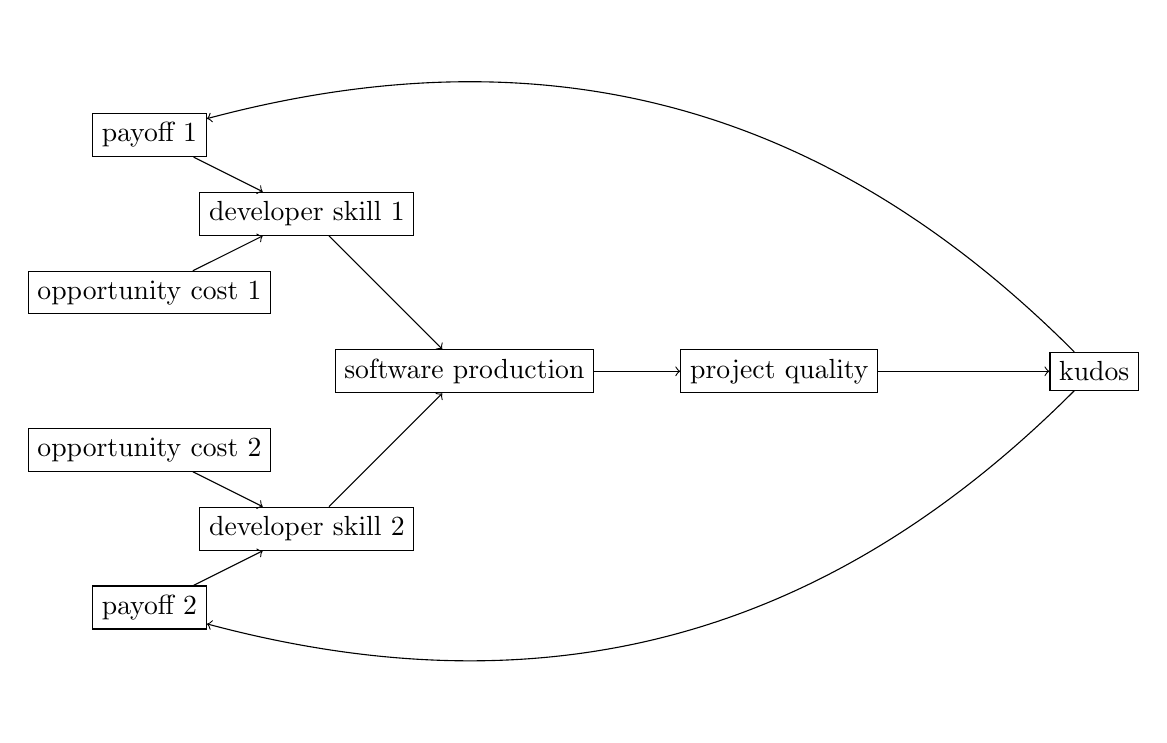
\begin{tikzpicture}
    % Nodes
    \node[draw, rectangle] (O1) at (2, 1) {opportunity cost 1};
    \node[draw, rectangle] (J1) at (2, 3) {payoff 1};
    \node[draw, rectangle] (J2) at (2, -3) {payoff 2};
    \node[draw, rectangle] (O2) at (2, -1) {opportunity cost 2};
    \node[draw, rectangle] (T1) at (4, 2) {developer skill 1};
    \node[draw, rectangle] (T2) at (4, -2) {developer skill 2};
    \node[draw, rectangle] (F) at (6, 0) {software production};
    \node[draw, rectangle] (Q) at (10, 0) {project quality};
    \node[draw, rectangle] (K) at (14, 0) {kudos};
    
    % Edges
    \draw[->] (O1) -- (T1);
    \draw[->] (J1) -- (T1);
    \draw[->] (O2) -- (T2);
    \draw[->] (J2) -- (T2);
    \draw[->, bend right] (K) to (J1);
    \draw[->, bend left] (K) to (J2);
    \draw[->] (F) -- (Q);
    \draw[->] (Q) -- (K);
    \draw[->] (T1) -- (F);
    \draw[->] (T2) -- (F);
\end{tikzpicture}
